% Name: Figure-eight knot
% Description: The figure-eight knot 4₁, drawn as one closed strand with four alternating crossings.
% Tags: figure-eight knot, knot, alternating

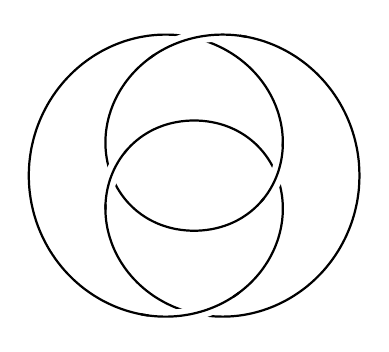
\begin{tikzpicture}[scale=0.7, knot/.style={domain=#1, samples=60, smooth, variable=\t}]
  % The curve ((2 + cos 2t) cos 3t, (2 + cos 2t) sin 3t) with height sin 4t, which crosses itself at t = 30°, 60°, 120°, 150°, 210°, 240°, 300°, and 330°
  \draw[thick, knot=0:360, samples=241] plot ({(2+cos(2*\t))*cos(3*\t)}, {(2+cos(2*\t))*sin(3*\t)});
  % The strand on top at each crossing is the one where sin 4t > 0: t = 30°, 120°, 210°, and 300°
  \foreach \c in {30, 120, 210, 300} {
    \draw[white, line width=5pt, knot=\c-6:\c+6] plot ({(2+cos(2*\t))*cos(3*\t)}, {(2+cos(2*\t))*sin(3*\t)});
    \draw[thick, knot=\c-7:\c+7] plot ({(2+cos(2*\t))*cos(3*\t)}, {(2+cos(2*\t))*sin(3*\t)});
  }
\end{tikzpicture}
